% We will implement the SpectralEmbedding method (also provided by Datafold) with the same settings as those detailed in the paper.

% \textbf{Spectral Embedding}

In this exercise, we will handle multidimensional and large datasets, the details of which will be elaborated upon. To address the challenge of dimensionality reduction, we will employ a method known as Spectral Embedding. This technique is particularly effective for complex, non-linear data structures, as it utilizes the spectral properties of data. In fact, Spectral Embedding is similar to Diffusion Maps formerly explained and finds applications in clustering, visualization, and dimensionality reduction tasks. Spectral Embedding also works by constructing a matrix to represent the affinities or relationships between data points, followed by an analysis of the matrix's spectrum, specifically its eigenvalues and eigenvectors, to achieve dimensionality reduction. However, compared to Diffusion Maps, the emphasis on different eigenvectors (we might choose eigenvectors corresponding to the smallest eigenvalues, which capture the global structure of the data, rather than the fastest decaying eigenvalues as in Diffusion Maps) may lead to subtle differences in the resulting embeddings and their interpretability.

This method is supported by various Python libraries dedicated to manifold learning, including \texttt{scikit-learn} \cite{pedregosa2011scikit}, \texttt{Megaman} \cite{megaman}, and \texttt{Datafold} \cite{Lehmberg2020}. Our implementation will focus on \texttt{Datafold} for Spectral Embedding, which will then be compared with the implementation in \texttt{Megaman}.\\

% Megaman: SpectralEmbedding implements Diffusion Maps (Nadler et al., 2006): This method uses the eigendecomposition of the Laplacian.

Megaman is a scalable manifold learning package developed in Python, designed particularly for large data sets. Megaman's API is designed to be familiar to users of scikit-learn, inheriting much of its functionality. This makes it easier for those already accustomed to scikit-learn to adapt to Megaman. It requires standard Python libraries like NumPy, SciPy, and scikit-learn to function. Megaman utilizes the C++ Fast Library for Approximate Nearest Neighbors (FLANN) and the Sparse Symmetric Positive Definite (SSPD) solver Locally Optimal Block Preconditioned Gradient (LOBPCG) method. An overview of the classes and packages used can be seen in Fig. \ref{fig:megaman}. The self-implemented classes are depicted in gray, framed, while packages are in gray, with no frame, and external packages in blue.

\begin{figure}[H]
    \centering
    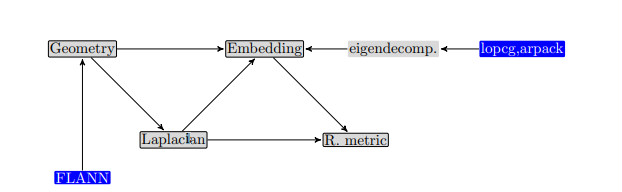
\includegraphics[width=0.8\linewidth]{images/megamen.png}
    \caption{Understanding Megaman}
    \label{fig:megaman}
\end{figure}

These advanced tools help in scaling manifold learning algorithms for handling large datasets efficiently. Megaman is specifically designed for high performance and research purposes. Megaman caches intermediary steps and indices, facilitating fast re-computation with new parameters, a valuable feature for experimental and iterative research work. The package implements several manifold learning algorithms in its own classes, which inherit from a base class. These include \texttt{SpectralEmbedding}, LTSA, LocallyLinearEmbedding, and Isomap. Each of these algorithms has its own significance and applications in manifold learning. We are going to focus on \texttt{SpectralEmbedding}, which, as stated earlier in the paper, is a manifold learning technique that typically deals with the graph structure of the data, focusing on capturing the essence of the data in fewer dimensions by using the eigenvectors of the Laplacian matrix. The matrix's eigenvalues and eigenvectors are then computed, with the eigenvectors corresponding to the smallest non-zero eigenvalues serving as the new data representation. This preserves local pairwise distances, making it particularly effective for data that lies on a curved manifold. Spectral embedding focuses on the graph structure directly without simulating a diffusion process over time.

The Geometry class in Megaman implements geometric operations common to many embedding algorithms, such as computing distances and Laplacians. This class enhances the versatility and applicability of the package in manifold learning tasks. The RiemannianMetric feature in Megaman estimates the Riemannian metric, enhancing the precision of manifold learning. Moreover, the eigendecomposition module provides a unified interface to various eigendecomposition methods available in SciPy, streamlining the process of implementing these methods. \\

We will compare the spectral embedding method with \texttt{Datafold}'s diffusion maps. Datafold is a Python package that provides data-driven models for point clouds to find an explicit manifold parametrization and to identify non-linear dynamical systems on these manifolds. The explicit data manifold treatment allows prior knowledge of a system and its problem-specific domain to be included. Especially, Datafold utilizes diffusion maps for non-linear dimension reduction to reveal geometric structures within data. This technique defines a diffusion process on data, simulating how points interact over time, and employs eigenfunctions to capture these dynamics. The alpha parameter adjusts the approach, aligning it with mathematical concepts like the Graph Laplacian. Datafold's implementation, found in the \texttt{datafold.dynfold.DiffusionMaps} class, supports diverse data formats and includes features like inverse transformations for mapping from the reduced dimensional space back to the original space. Diffusion maps, as a manifold learning strategy, are part of the spectral methods family but are unique in their focus on data's diffusion properties.

That's why we decided to compare the different libraries and algorithms. 



